\documentclass[12pt]{article}


\usepackage[portuguese]{babel}
\usepackage[utf8]{inputenc}
\usepackage[textwidth=17.5cm]{geometry}
\usepackage{listings}
\usepackage{tikz}
\usepackage{booktabs}
\usepackage[linguistics]{forest}
\usepackage{float}
\usepackage{indentfirst}
\usepackage{titlesec}
\usepackage{amsmath}
\usepackage{subcaption}
\usepackage{hyperref}
\usepackage{textcomp}
\usepackage[most]{tcolorbox}
\usepackage{lipsum}
\usepackage{fancyvrb}


\title{
    \Huge Processamento de Linguagens\\
    \normalsize \textbf{Trabalho Prático 1}
}

\date{\today}

\setlength{\parindent}{2em}

\begin{document}

\begin{titlepage}

    \maketitle
    \begin{center}\large

        \begin{tabular}{ll}
            \textbf{Grupo} nr. & 36
            \\\hline
            a83899 & André Morais
            \\
            a85954 & Luís Ribeiro
            \\
            a84783 & Pedro Rodrigues
        \end{tabular}

    \end{center}

    \vfill

    \begin{figure}[h]
        \centering
        
\includegraphics[height=3cm]{images/UM.png}
    \end{figure}

    \begin{center}
        \large Mestrado Integrado em Engenharia Informática\\
        Universidade do Minho
    \end{center}

\end{titlepage}

\tableofcontents{}

\newpage

\section{Introdução}

\vspace{1cm}

\subsection{Contexto}

\vspace{0.5cm}

Este relatório foi produzido em conformidade com a UC de \textbf{Processamento de Linguagens}, correspondente ao segundo semestre do terceiro ano do Mestrado Integrado em Engenharia Informática da Universidade do Minho.\\

\subsection{Problema}

\vspace{0.5cm}

Para vários projetos de desenvolvimento, é habitual haver soluções envolvendo vários ficheiros e várias pastas, como \texttt{Makefile}, \texttt{README} ou uma paste de exemplos.

Pretende-se, então, criar um programa \textbf{mkfromtemplate}, capaz de aceitar um nome de projeto e um ficheiro de descrição (template) e que crie os ficheiros e as pastas do peojeto, bem como escreva o conteúdo dos ficheiros pretendido.

O template deverá ser constituído por:
\begin{itemize}
  \item metadados (author e email)
  \item tree (estrutura de diretorias e ficheiros a criar)
  \item template de cada ficheiro
\end{itemize}

Um exemplo do template pode ser encontrado em \ref{tflex}.\\

\subsection{Objetivos}

\vspace{0.5cm}

Este projeto tem como principais objetivos:

\begin{itemize}
    \item aumentar a experiência de uso do ambiente \texttt{Linux} e de algumas ferramentas de apoio à programação;
    \item aumentar a capacidade de escrever \textit{Expressões Regulares (\textbf{ER})} para descrição de \textit{padrões de frases};
    \item desenvolver, a partir de ERs, sistemática e automaticamente \textit{Processadores de Linguagens Regulares, que filtrem ou transformem textos com base no conceito de regras de produção \textit{Condição-Ação}};
    \item utilizar o Flex para gerar \textit{filtros} de texto em C.
\end{itemize}

\newpage

\section{Análise e Especificação}

\vspace{1cm}

Após uma análise ao problema, consegue-se identificar uma série de requisitos necessários para a resolução do problema.

\subsection{Requisitos:}

\vspace{0.5cm}

\begin{itemize}
    \item Alterar nome das variáveis no ficheiro template;
    \item Identificar os diferentes tipos de dados do template (meta, tree e conteúdo de cada ficheiro);
    \item Guardar em memória, numa estrutura de dados adequada, a informação acerca da estrutura do projeto (\textit{tree} de ficheiros e pastas).
    \item Utilizar a estrutura de dados e a informação guardada para criar a estrutura final.
\end{itemize}

\vspace{1cm}

\section{Concepção e Codificação da Resolução}

Observando o problema e os requisitos, precisamos, primeiramente, de alterar o nome das variáveis. Para isto foi utilizado um filtro flex especialemente para alterar o nome destas variáveis. O processo é simples, é criada uma HashTable, usando as bibliotecas da glib, onde é guardada a informação de cada metadado, da forma (Chave, Valor).

\textbf{Exemplo}:

\indent\indent\texttt{author: Pedro}  $\rihtarrow$ gera um par (auhtor, Pedro).

\vspace{0.5cm}
\begin{tcolorbox}
\begin{verbatim}
<META>^[a-zA-Z0-9_]+/:[ ]        {key=strdup(yytext);BEGIN VALUE;}
<VALUE>[^\n]*      {value=strdup(yytext+2);addToTable(key,value);BEGIN META;}
\end{verbatim}
\end{tcolorbox}

Para tal, era necessário diferenciar o grupo \texttt{METADADOS} dos restantes grupos (onde serão substituídas as variáveis). O mais sensato é utilizar uma \textit{start condition} como mostramos a seguir:

\vspace{0.5cm}
\begin{tcolorbox}
\begin{verbatim}
<*>\{%/[a-zA-Z0-9_]+%\}     {BEGIN SUBS;}
^===[ ]meta                 {initializeHash();BEGIN META;}
<SUBS>{
[a-zA-Z0-9_]+/%\}           {printf(getValue(yytext));}
%\}                         {BEGIN TF;}
}
<META>^===[ ]tree           {ECHO;BEGIN TF;}
\end{verbatim}
\end{tcolorbox}

Com este filtro, obteremos o nosso template com todas as variáveis alteradas para o seu respetivo nome e sem o grupo \texttt{METADADOS}, uma vez que este é inútil nesta fase do processo.

Agora, temos um ficheiro totalmente útil para começar a estruturar o projeto. O primeiro passo é descobrir como identificar os diferentes grupos do ficheiro template (tree de ficheiros e pastas e conteúdo de ficheiros).

Tal como no requisito anterior, o mais sensato a utilizar é \textit{start conditions} e identificar a expressão regular que apanhe o inicio e fim de cada grupo:


\begin{tcolorbox}
\begin{verbatim}
^===[  ]tree                {initializeTree();BEGIN TREE;}
<TREE>{
[^\n\\\*\?\<\>\|\/]+\/$     {insertDir(yytext);BEGIN PROF;}
[^\n\\\*\?\<\>\|\/]+        {insertFile(yytext);BEGIN PROF;}
.|\n                        {;}
}
<PROF>{
^===[  ][^\n]+              {makeTree();file=strdup(yytext+4);BEGIN FILES;}
^-+[  ]                     {nprof=strlen(yytext)-1;BEGIN TREE;}
.|\n                        {;}
}
<FILES>{
^===[ ][^\n]+               {file=strdup(yytext+4);}
^[^\n]*                     {writef(yytext,file);}
^\n                         {writef("",file);}
.|\n                        {;}
}
.|\n                        {;}

\end{verbatim}
\end{tcolorbox}

Como se pode reparar, é apresentada uma \textit{start condition} que não era espectável: \textbf{PROF}. Esta é necessária para calcular a profundidade de um ficheiro na árvore.

Com estes pedaços de código, resolve-se o problema de identificar os grupos distintos presentes no ficheiro. No entanto, é preciso iterar sobre a informação presente em cada grupo.\\

Respeitando o que foi enunciado nos requisitos, é necessário decidir a estrutura de dados que mais se adequa para guardar a informação da localização de cada ficheiro, e, tal como o nome do grupo (\textit{tree}) indica, a melhor estrutura de dados a ser usada é uma árvore, mais concretamente uma \texttt{N-ARY TREE}, ou seja, uma árvore em que cada nodo pode ter N nodos. Assim, para o ficheiro template de exemplo apresentado e com nome de projeto \textit{flex}, a árvore seria representada da seguinte forma:

\begin{figure}[H]
\centering
    \begin{forest}
    \Tree[./
            [flex/
                [doc/
                    [flex.md]
                ]
                [exemplo/]
                [flex.fl]
                [Makefile]
                [README]
            ]
        ]
    \end{forest}
\end{figure}

Após uma análise no mundo da internet, encontra-se uma implementação deste tipo de árvores apresentada pela \texttt{GLIB}, que pode ser usada para representar este tipo de problema.

Depois de obtida uma implementação desta árvore, é trivial que o próximo passo é identificar o tipo de nodo que será adicionado (ficheiro ou diretoria) e guardar o nome na profundidade certa da árvore.

\begin{verbatim}
GNode* addToTree(char* nome, int file, GNode* parent){
    Node* new = malloc(sizeof(struct node));
    new->descricao = strdup(nome);
    new->file = file;
    GNode* node;
    if (parent==NULL){
        node = g_node_new(new);
        g_node_append(dirs,node);
    }
    else{
        node = g_node_new(new);
        g_node_append(parent,node);
    }
    return node;
}

void insertDir(char* nome){
    while(nprof!=prof){
        parent=parent->parent;
        prof--;
    }
    parent=addToTree(nome,0,parent);
    prof++;
    nprof=0;
}

void insertFile(char* nome){
    while(nprof!=prof){
        parent=parent->parent;
        prof--;
    }
    addToTree(nome,1,parent);
    nprof=0;
}
\end{verbatim}

Neste algoritmo é importante salientar que \textit{prof} representa a \textbf{profundidade da última diretoria criada} e \textit{nprof} representa a \textbf{profundidade da diretoria ou ficheiro a ser criado}.

Estas funções escritas em C, são chamadas quando são identificadas pelas expressões regulares apresentadas no código anterior a este.

Com a árvore completa, o processo de criação de pastas e ficheiros é trivial.

\begin{verbatim}
void transformTree (GNode* dir,char* path){
    if (dir!=NULL){
        GNode* child = g_node_first_child(dir);
        char command [1024];
        while(child){
            Node* dados = child->data;
            if (dados->file) sprintf(command,"touch %s%s",path,dados->descricao);
            else sprintf(command,"mkdir %s%s",path,dados->descricao);
            system(command);
            if (!dados->file){
                sprintf(command,"%s%s",path,dados->descricao);
                transformTree(child,command);
            }
            child=child->next;
        }
    }
}


void makeTree(){
    char pwd [64];
    getcwd(pwd,sizeof(pwd));
    strcat(pwd,"/");
    transformTree(dirs,pwd);
}
\end{verbatim}

Seguindo, novamente, a estrutura criada nos requisitos, o próximo passo é processar esta informação presente na árvore. Para tal, é necessário, primeiro, encontrar as expressões regulares que apanham o nome do ficheiro a editar.

\begin{tcolorbox}
\begin{verbatim}
^===[ ][^\n]+                               {file=strdup(yytext+4);}
^[^\n]+                                     {writef(yytext,file);}
^\n                                         {writef("",file);}
\end{verbatim}
\end{tcolorbox}

Com as ERs apresentadas em cima, obtemos o nome do ficheiro em \textit{file} e conseguimos escreeer o resultado do yytext nesse mesmo ficheiro.

\begin{verbatim}
int getFilePath (GNode* dir,char* f,char* path){
    if (dir!=NULL){
        GNode* child = g_node_first_child(dir);
        while(child){
            Node* dados = child->data;
            if (dados->file){
                if (strcmp(dados->descricao,f)==0){
                    strcat(path,f);
                    return 1;
                }
            }
            else{
                strcat(path,dados->descricao);
                if (getFilePath(child,f,path)==1) return 1;
                else{
                    int nc = strlen(path)-strlen(dados->descricao);
                    path[nc]='\0';
                }
            }
            child=child->next;
        }
    }
    return 0;
}



int writef (char* s, char* f){
    char path [1024];
    getcwd(path,sizeof(path));
    strcat(path,"/");
    if (getFilePath(dirs,f,path)==1){
        FILE *f = fopen(path,"a");
        fprintf(f,"%s\n",s);
        fclose(f);
    }
    return 0;
}
\end{verbatim}

Com todo o processo enunciado anteriormente, obtém-se dois filtros distintos que precisam de ser encadeados. O segundo deverá processar o resultado do primeiro, que por sua vez processa o texto enviado como argumento.
Uma opção é criar definir o prefixo de cada um dos filtros e criar um programa em c que junte os dois.
Para simplificar as coisas, define-se o primeiro filtro de alteração de variáveis como \texttt{vars} e o responsável por criar as diretorias e ficheiros como \texttt{tmpl}. Isto faz com que sejam obtidas duas funções (\textbf{varslex()} e \textbf{tmpllex()}) que podem ser usadas para chamar os respetivos filtros em C.

O processo de junção destes dois filtros deverá seguir os seguintes passos:

\vspace{0.5cm}

\textbf{Primeira fase:}
\begin{enumerate}
    \item Redirecionar stdout para ficheiro temporário (pipe)
    \item Redirecionar stdin para ficheiro recebido como argumento
    \item Correr o primeiro filtro para alterar as variáveis com a função \texttt{varslex()}
    \item Redirecionar o stdin e stdout para os descritores originais
\end{enumerate}

\textbf{Segunda fase:}
\begin{enumerate}
    \item Redirecionar stdin para o ficheiro temporário (pipe)
    \item Correr o segundo filtro para criar diretorias e ficheiros com a função \texttt{tmpllex()}
    \item Redirecionar o stdin para o descritor original
    \item Elimiar o ficheiro temporário (pipe)
\end{enumerate}


\newpage

\section{Testes e Resultados}

Para testar o programa foram criados três ficheiros template:

\begin{itemize}
    \item Template para projeto em Flex - \ref{tflex}
    \item Template para projeto em C - \ref{tc}
    \item Template à procura de bugs na definição de meta e tree - \ref{tb}
\end{itemize}

Os ficheiros de testes serão apresentados no anexo.

\newpage

\subsection{Teste 1 - Flex}

\begin{figure}[H]
    \centering
    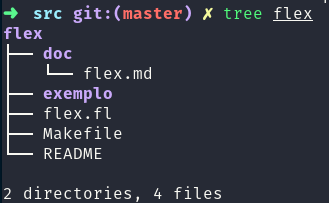
\includegraphics[width=0.5\linewidth]{images/tflex.png}
    \caption{Árvore de diretorias e ficheiros criados}
\end{figure}

\begin{figure}[H]
    \centering
    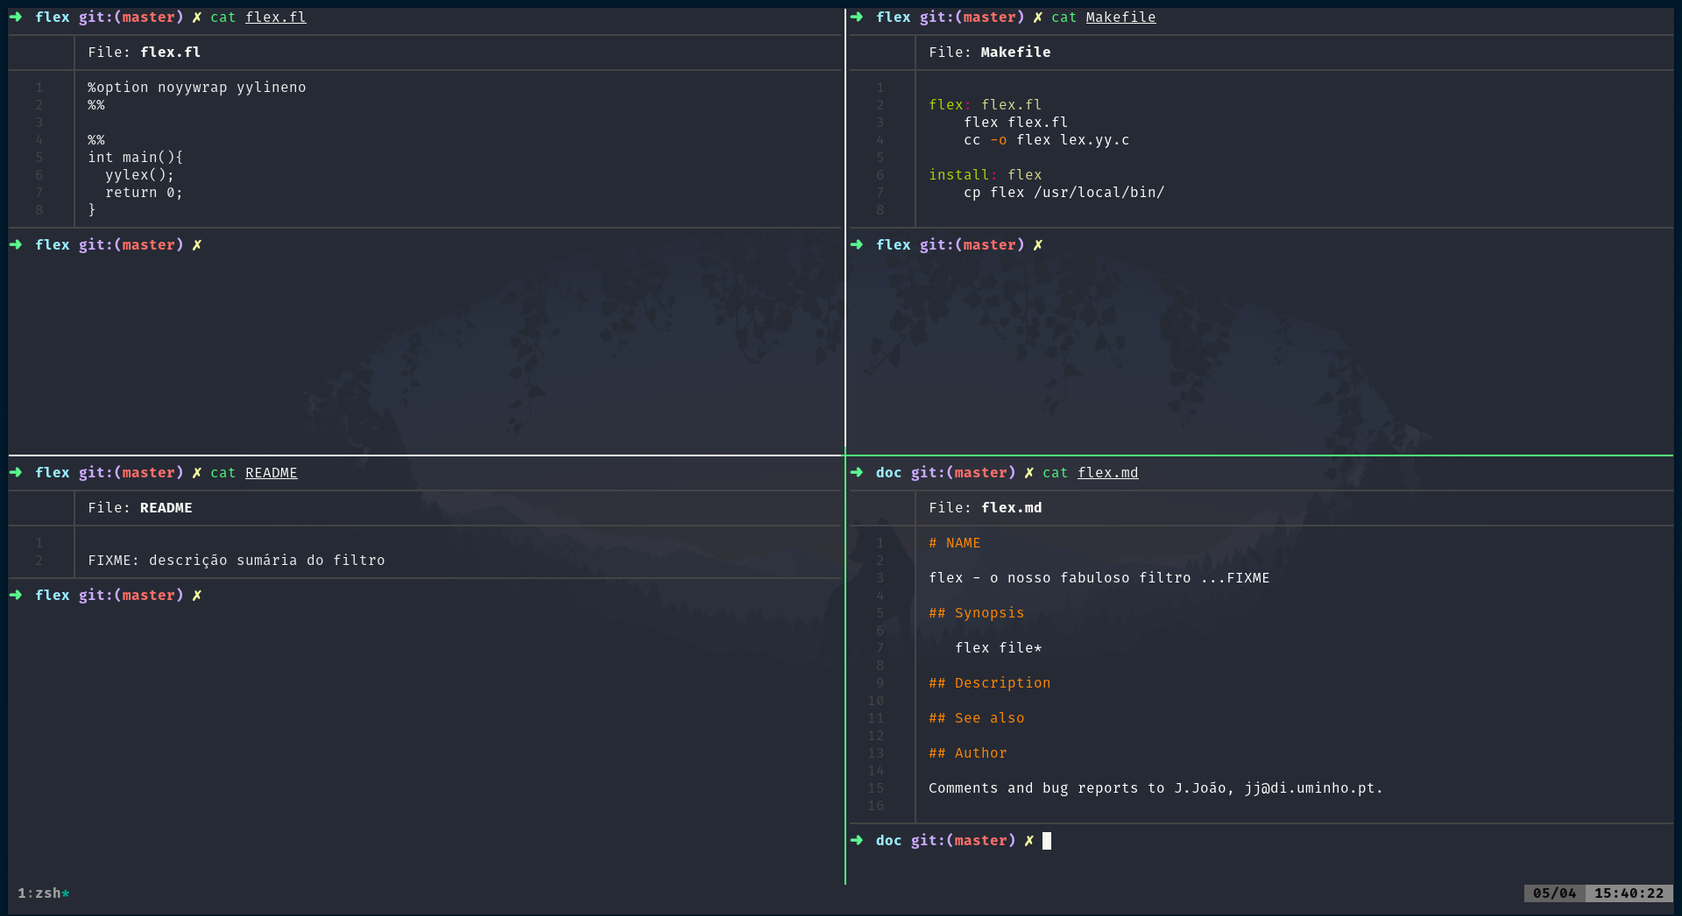
\includegraphics[width=\linewidth]{images/fflex.png}
    \caption{Conteúdo dos ficheiros criados}
\end{figure}

\subsection{Teste 2 - C}

\begin{figure}[H]
    \centering
    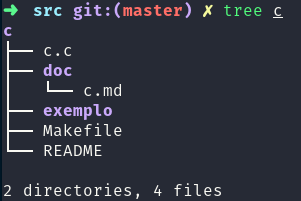
\includegraphics[width=0.5\linewidth]{images/tc.png}
    \caption{Árvore de diretorias e ficheiros criados}
\end{figure}

\begin{figure}[H]
    \centering
    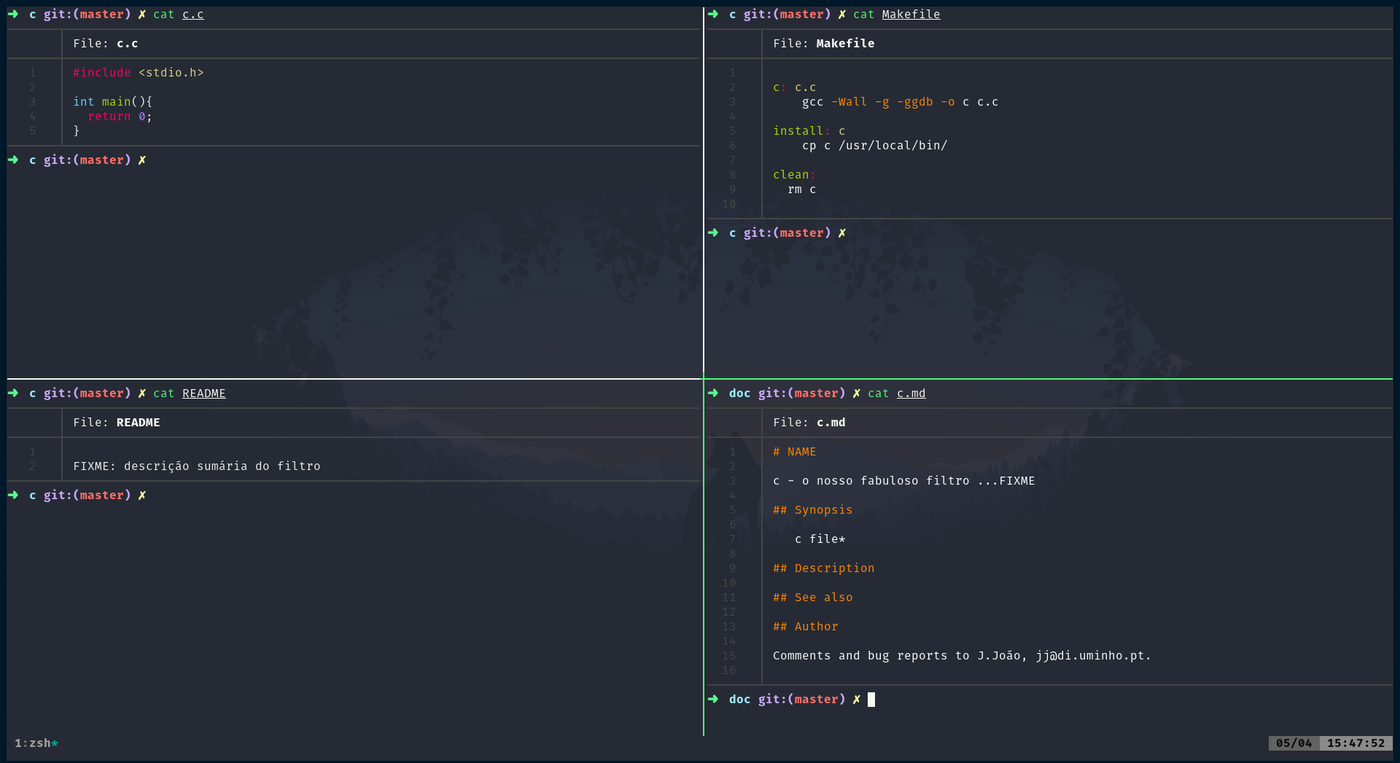
\includegraphics[width=\linewidth]{images/fc.png}
    \caption{Conteúdo dos ficheiros criados}
\end{figure}

\subsection{Teste 3 - Check Bugs}

\begin{figure}[H]
    \centering
    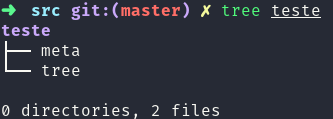
\includegraphics[width=0.5\linewidth]{images/tb.png}
    \caption{Árvore de diretorias e ficheiros criados}
\end{figure}

\begin{figure}[H]
    \centering
    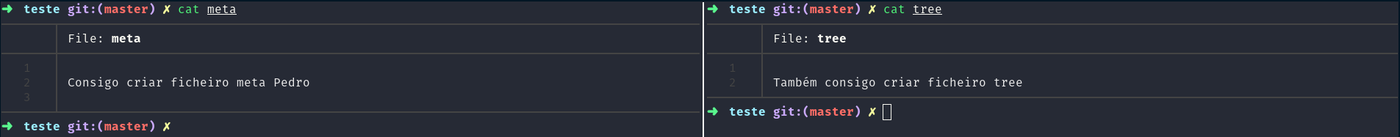
\includegraphics[width=\linewidth]{images/fb.png}
    \caption{Conteúdo dos ficheiros criados}
\end{figure}

\newpage

\section{Conclusão}

Depois de terminado o primeiro trabalho prático da Unidade Curricular de Processamento de Linguagens, concluímos que a realização deste permitiu-nos consolidar os conhecimentos estudados nas aulas da disciplina. Houve assim, uma aprendizagem notória relativamente ao analisador léxico (flex) e às suas funcionalidades, desde as Expressões Regulares (ERs) iniciais até ao uso de Start Conditions e look-aheads.

O uso da biblioteca Glib ajudou-nos bastante na parte da estruturação de memória, pois esta fornece estruturas de dados, tais como a GTree e a GHashTable, e funções relativas a essas estruturas.

Em jeito de conclusão, consideramos o nosso desempenho bastante satisfatório, pois foi possível responder a todas as questões pedidas pelo docente e os objetivos foram concluídos.

\newpage

\appendix
\section{Código do Programa}

\subsection{vars.fl}
\VerbatimInput{./../src/vars.fl}

\newpage

\subsection{filtro.fl}
\VerbatimInput{./../src/filtro.fl}

\newpage

\subsection{template.c}
\VerbatimInput{./../src/template.c}

\newpage

\subsection{Template Flex}
\label{tflex}
\VerbatimInput{./../src/templates/template-flex}

\newpage

\subsection{Template C}
\label{tc}
\VerbatimInput{./../src/templates/templatec}

\newpage

\subsection{Template para procurar bugs em meta e tree}
\label{tb}
\VerbatimInput{./../src/templates/templateTeste}
\end{document}g
